% $Author: oscar $
% $Date: 2009-09-15 16:53:48 +0200 (Tue, 15 Sep 2009) $
% $Revision: 29111 $
%=================================================================
\ifx\wholebook\relax\else
% --------------------------------------------
% Lulu:
	\documentclass[a4paper,10pt,twoside]{book}
	\usepackage[
		papersize={6.13in,9.21in},
		hmargin={.815in,.815in},
		vmargin={.98in,.98in},
		ignoreheadfoot
	]{geometry}
	\usepackage[hangul]{kotex}
	% $Author: oscar $
% $Date: 2009-09-13 20:58:29 +0200 (Sun, 13 Sep 2009) $
% $Revision: 29070 $
%=============================================================
% NB: documentclass must be set in main document.
% Allows book to be generated in multiple formats.
%=============================================================
%:Packages
\usepackage[T1]{fontenc}  %%%%%really important to get the code directly in the text!
\usepackage{palatino}
\usepackage{ifthen}
\usepackage{graphicx}
\graphicspath{{figures/}}
\usepackage{xspace}
\usepackage{makeidx}
\usepackage{isodateo} % enable \isodate
\usepackage{amssymb,textcomp}
%=============================================================
%:More packages
%\usepackage[english]{babel}
%\usepackage{lmodern}
%\usepackage[scaled=0.85]{helvet}
%\usepackage{microtype}
%\usepackage{theorem}
%\usepackage{float}
%\usepackage{longtable}
%\usepackage[nottoc]{tocbibind}
%\usepackage{multicol}
%\usepackage{booktabs}	% book-style tables
%\usepackage{topcapt}	% enables \topcaption
%\usepackage{multirow}
%\usepackage{tabularx}
%\usepackage{alltt}
\usepackage[usenames,dvipsnames]{color}
%\usepackage[hang]{subfigure}\makeatletter\def\p@subfigure{\thefigure\,}\makeatother
%\usepackage{rotating}
%\usepackage{enumitem}	% apb: allows more control over tags in enumerations
%\usepackage{verbatim}     % for comment environment
%\usepackage{varioref}	% for page references that work
%\usepackage{needspace}
%\usepackage[newparttoc]{titlesec}
%\usepackage{titletoc}
%\usepackage{wrapfig}
\usepackage[
	colorlinks=true,
	linkcolor=black,
	urlcolor=black,
	citecolor=black
]{hyperref}   % should come last
%=============================================================
%:URL style
\makeatletter
\def\url@leostyle{%
  \@ifundefined{selectfont}{\def\UrlFont{\sf}}{\def\UrlFont{\sffamily}}}
\makeatother
\urlstyle{leo}
%=============================================================
%:Booleans
\newboolean{lulu}
\setboolean{lulu}{false}
\newcommand{\ifluluelse}[2]{\ifthenelse{\boolean{lulu}}{#1}{#2}}
%=============================================================
%:Editorial comment macros
\newcommand{\nnbb}[2]{
  \fbox{\bfseries\sffamily\scriptsize#1}
  {\sf\small$\blacktriangleright$\textit{#2}$\blacktriangleleft$}
}
\newcommand{\on}[1]{\nnbb{Oscar}{#1}}
\newcommand{\here}{\nnbb{CONTINUE}{HERE}}
%=============================================================
%:Abbreviation macros
\newcommand{\ie}{\emph{i.e.},\xspace}
\newcommand{\eg}{\emph{e.g.},\xspace}
\newcommand{\etc}{\emph{etc.}\xspace}
\newcommand{\etal}{\emph{et al.}\xspace}
\newcommand{\straightquote}{"}
\newcommand{\sba}{\url{SquareBracketAssociates.org}\xspace}
%=============================================================
%:Patterns
% \newcommand{\pattern}[2]{\newpage\section{{\sf #1}}\label{pat:#2}}
% \newcommand{\pattern}[2]{\newpage\index{#1 (Pattern)}\section{#1}\label{pat:#2}}
\newcommand{\pattern}[2]{\cleardoublepage\index{#1 (패턴)}\section{#1}\label{pat:#2}}
\newcommand{\thumbnail}[2]{\index{#1 (패턴)}\subsection{#1}\label{pat:#2}}
\newcommand{\thumblang}[2]{\index{#1 (패턴 랭귀지)}\subsection{#1}\label{pat:#2}}
\newcommand{\variant}[1]{{\emph{#1}}\xspace}
% \newcommand{\problem}[1]{\subsection*{Problem}\emph{#1}}
\newcommand{\intent}[1]{\paragraph{의도}\emph{#1}}
\newcommand{\problem}[1]{\paragraph{문제}\emph{#1}}
\newcommand{\solution}[1]{\paragraph{해결}\emph{#1}}
\newcommand{\discussion}[0]{\paragraph{토론}}
\newcommand{\cmd}[1]{{\tt #1}\xspace}
%=============================================================
%:Environments
\newenvironment{bulletlist}{\begin{itemize}\setlength{\itemsep}{0ex}}
{\end{itemize}}
%=============================================================
%:Cross reference macros
\newcommand{\chalabel}[1]{\label{cha:#1}}
\newcommand{\seclabel}[1]{\label{sec:#1}}
\newcommand{\figlabel}[1]{\label{fig:#1}}
\newcommand{\tablabel}[1]{\label{tab:#1}}
\newcommand{\rulelabel}[1]{\label{rule:#1}}
\newcommand{\eglabel}[1]{\label{eg:#1}}
\newcommand{\scrlabel}[1]{\label{scr:#1}}
\newcommand{\mthlabel}[1]{\label{mth:#1}}
\newcommand{\clslabel}[1]{\label{cls:#1}}
\newcommand{\faqlabel}[1]{\label{faq:#1}}
%\newcommand{\charef}[1]{Chapter~\ref{cha:#1}\xspace}
%\newcommand{\secref}[1]{Section~\ref{sec:#1}\xspace}
\newcommand{\figref}[1]{Figure~\ref{fig:#1}\xspace}
% \newcommand{\patpgref}[2]{\hyperref[pat:#2]{\sf #1} [p.~\pageref{pat:#2}]\xspace}
\newcommand{\patpgref}[2]{\index{#1 (Pattern)}\hyperref[pat:#2]{#1} [p.~\pageref{pat:#2}]\xspace}
\newcommand{\patlangpgref}[2]{\index{#1 (Pattern language)}\hyperref[pat:#2]{#1} [p.~\pageref{pat:#2}]\xspace}
% \newcommand{\patref}[2]{\hyperref[pat:#2]{\sf #1}\xspace}
\newcommand{\patref}[2]{\index{#1 (Pattern)}\hyperref[pat:#2]{#1}\xspace}
\newcommand{\patlangref}[2]{\index{#1 (Pattern language)}\hyperref[pat:#2]{#1}\xspace}
% \newcommand{\charef}[2]{\hyperref[cha:#2]{\underline{\sf #1}}\xspace}
% \newcommand{\charef}[2]{\hyperref[cha:#2]{\sf #1}\xspace}
\newcommand{\charef}[2]{\index{#1 (Pattern cluster)}\hyperref[cha:#2]{#1}\xspace}
% \newcommand{\chapgref}[2]{\hyperref[cha:#2]{\sf #1} [p.~\pageref{cha:#2}]\xspace}
\newcommand{\chapgref}[2]{\index{#1 (Pattern cluster)}\hyperref[cha:#2]{#1} [p.~\pageref{cha:#2}]\xspace}
%\newcommand{\Figref}[1]{Figure~\ref{fig:#1}\xspace}
%\newcommand{\appref}[1]{Appendix~\ref{app:#1}\xspace}
%\newcommand{\tabref}[1]{Table~\ref{tab:#1}\xspace}
%\newcommand{\ruleref}[1]{\ref{rule:#1}\xspace}
%\newcommand{\egref}[1]{example~\ref{eg:#1}\xspace}
%\newcommand{\Egref}[1]{Example~\ref{eg:#1}\xspace}
%\newcommand{\scrref}[1]{script~\ref{scr:#1}\xspace}
%\newcommand{\Scrref}[1]{Script~\ref{scr:#1}\xspace}
%\newcommand{\tscrref}[1]{the script~\ref{scr:#1}\xspace}
%\newcommand{\Tscrref}[1]{The script~\ref{scr:#1}\xspace}
%\newcommand{\mthref}[1]{method~\ref{mth:#1}\xspace}
%\newcommand{\mthsref}[1]{methods~\ref{mth:#1}\xspace}
%\newcommand{\Mthref}[1]{Method~\ref{mth:#1}\xspace}
%\newcommand{\tmthref}[1]{the method~\ref{mth:#1}\xspace}
%\newcommand{\Tmthref}[1]{The method~\ref{mth:#1}\xspace}
%\newcommand{\clsref}[1]{class~\ref{cls:#1}\xspace}
%\newcommand{\tclsref}[1]{the class~\ref{cls:#1}\xspace}
%\newcommand{\Tclsref}[1]{The class~\ref{cls:#1}\xspace}
%=============================================================
%:Page Layout
\setlength{\headsep}{1cm}
%=============================================================
%:Menu item macro
%\definecolor{lightgray}{gray}{0.89}
%\newcommand{\menu}[1]{{%
%	\setlength{\fboxsep}{0pt}%
%	\colorbox{lightgray}{{{\upshape\sffamily\strut \,#1\,}}}}}
%\newcommand{\go}{\,$\triangleright$\,}
%\newcommand{\short}[1]{\mbox{{\sc cmd}\hspace{0.08em}--\hspace{0.09em}#1}\xspace}
%\newcommand{\button}[1]{{%
%	\setlength{\fboxsep}{0pt}%
%	\fbox{{\upshape\sffamily\strut \,#1\,}}}}
%\newcommand{\toolsflap}{\textit{Tools} flap\xspace}
%=============================================================
%:Section depth
%\setcounter{secnumdepth}{2}
%
%\DeclareGraphicsExtensions{.pdf, .jpg, .png}
%=============================================================
%:PDF setup
\hypersetup{
   pdftitle={Object-Oriented Reengineering Patterns},
   pdfauthor={Serge Demeyer, St\'ephane Ducasse, Oscar Nierstrasz},
   pdfkeywords={Reengineering, Object-Oriented Programming, Patterns},
   pdfsubject={Computer Science}
}
%=============================================================
%:Page layout and appearance
%\renewcommand{\chaptermark}[1]{\markboth{#1}{}}
%\renewcommand{\sectionmark}[1]{\markright{\thesection\ #1}}
%\renewpagestyle{plain}[\small\itshape]{%
%	\setheadrule{0pt}%
%	\sethead[][][]{}{}{}%
%	\setfoot[][][]{}{}{}}
%\renewpagestyle{headings}[\small\itshape]{%
%	\setheadrule{0pt}%
%	\setmarks{chapter}{section}%
%	\sethead[\thepage][][\chaptertitle]{\sectiontitle}{}{\thepage}%
%	\setfoot[][][]{}{}{}}
%=============================================================
%:Title section setup and TOC numbering depth
%\setcounter{secnumdepth}{1}
%\setcounter{tocdepth}{1}
%\titleformat{\part}[display]{\centering}{\huge\partname\ \thepart}{1em}{\Huge\textbf}[]
%\titleformat{\chapter}[display]{}{\huge\chaptertitlename\ \thechapter}{1em}{\Huge\raggedright\textbf}[]
%\titlecontents{part}[3pc]{%
%		\pagebreak[2]\addvspace{1em plus.4em minus.2em}%
%		\leavevmode\large\bfseries}
%	{\contentslabel{3pc}}{\hspace*{-3pc}}
%	{}[\nopagebreak]
%\titlecontents{chapter}[3pc]{%
%		\pagebreak[0]\addvspace{1em plus.2em minus.2em}%
%		\leavevmode\bfseries}
%	{\contentslabel{3pc}}{}
%	{\hfill\contentspage}[\nopagebreak]
%\dottedcontents{section}[3pc]{}{3pc}{1pc}
%\dottedcontents{subsection}[3pc]{}{0pc}{1pc}
%\let\origdoublepage\cleardoublepage
%\newcommand{\clearemptydoublepage}{%
%  \clearpage
%  {\pagestyle{empty}\origdoublepage}}
%\let\cleardoublepage\clearemptydoublepage % see http://www.tex.ac.uk/cgi-bin/texfaq2html?label=patch
%=============================================================
%:Listings package configuration
\newcommand{\caret}{\makebox{\raisebox{0.4ex}{\footnotesize{$\wedge$}}}}
% \newcommand{\escape}{{\sf \textbackslash}}
\definecolor{source}{gray}{0.95}
\usepackage{listings}
\lstdefinelanguage{Smalltalk}{
  morestring=[d]',
% Adapt this to other languages!
%  morecomment=[s]{"}{"},
  alsoletter={\#:},
  %escapechar={!},
  literate=
    {BANG}{!}1
%    {UNDERSCORE}{\_}1
    {\\st}{Smalltalk}9 % convenience -- in case \st occurs in code
    % {'}{{\textquotesingle}}1 % replaced by upquote=true in \lstset
%    {_}{{$\leftarrow$}}1
    {>>>}{{\sep}}1
    {^}{{$\uparrow$}}1
    {~}{{$\sim$}}1
    {-}{{\sf -\hspace{-0.13em}-}}1  % the goal is to make - the same width as +
    {+}{\raisebox{0.08ex}{+}}1		% and to raise + off the baseline to match -
    {-->}{{\quad$\longrightarrow$\quad}}3
	, % Don't forget the comma at the end!
  tabsize=4
}[keywords,comments,strings]

\lstset{language=Smalltalk,
	basicstyle=\sffamily,
	keywordstyle=\color{black}\bfseries,
	% stringstyle=\ttfamily, % Ugly! do we really want this? -- on
	mathescape=true,
	showstringspaces=false,
	keepspaces=true,
	breaklines=true,
	breakautoindent=true,
	backgroundcolor=\color{source},
	lineskip={-1pt}, % Ugly hack
	upquote=true, % straight quote; requires textcomp package
	columns=fullflexible} % no fixed width fonts
% \newcommand{\ct}{\lstinline[mathescape=false,basicstyle={\sffamily\upshape}]}
\newcommand{\ct}{\lstinline[mathescape=false,backgroundcolor=\color{white},basicstyle={\sffamily\upshape}]}
\newcommand{\lct}[1]{{\textsf{\textup{#1}}}}
%\newcommand{\scat}[1]{\emph{\textsf{#1}}\xspace}
%\newcommand{\prot}[1]{\emph{\textsf{#1}}\xspace}
% NB: No argument!
\lstnewenvironment{code}[0]{%
	\lstset{%
		% frame=lines,
		frame=single,
		framerule=0pt,
		mathescape=false
	}
}{}
%\def\ignoredollar#1{}
%=============================================================
%:Reserving space
%\newcommand{\needlines}[1]{\Needspace{#1\baselineskip}}
%=============================================================
%:Indexing macros
% Macros ending with "ind" generate text as well as an index entry
% Macros ending with "index" *only* generate an index entry
\newcommand{\ind}[1]{\index{#1}#1\xspace} % plain text
\newcommand{\subind}[2]{\index{#1!#2}#2\xspace} % show #2, subindex under #1
\newcommand{\emphind}[1]{\index{#1}\emph{#1}\xspace} % emph #1
\newcommand{\emphsubind}[2]{\index{#1!#2}\emph{#2}\xspace} % show emph #2, subindex under #1
\newcommand{\patind}[1]{\index{#1@#1 (pattern)}\ct{#1}\xspace} % pattern
\newcommand{\seeindex}[2]{\index{#1|see{#2}}} % #1, see #2
%\newcommand{\boldidx}[1]{{\bf #1}} % breaks hyperlink
%\newcommand{\indmain}[1]{\index{#1}#1\xspace} 
%\newcommand{\emphsubindmain}[2]{\index{#1!#2}\emph{#2}\xspace} % subindex, main entry
%\newcommand{\subindmain}[2]{\index{#1!#2}#2\xspace} % subindex, main entry
%\newcommand{\clsindmain}[1]{\index{#1!\#@(class)}\ct{#1}\xspace} % class main
%\newcommand{\indexmain}[1]{\index{#1}} 
%=============================================================
\parskip 1ex
%=============================================================

	\pagestyle{headings}
	\setboolean{lulu}{true}
% --------------------------------------------
% A4:
%	\documentclass[a4paper,11pt,twoside]{book}
%	% $Author: oscar $
% $Date: 2009-09-13 20:58:29 +0200 (Sun, 13 Sep 2009) $
% $Revision: 29070 $
%=============================================================
% NB: documentclass must be set in main document.
% Allows book to be generated in multiple formats.
%=============================================================
%:Packages
\usepackage[T1]{fontenc}  %%%%%really important to get the code directly in the text!
\usepackage{palatino}
\usepackage{ifthen}
\usepackage{graphicx}
\graphicspath{{figures/}}
\usepackage{xspace}
\usepackage{makeidx}
\usepackage{isodateo} % enable \isodate
\usepackage{amssymb,textcomp}
%=============================================================
%:More packages
%\usepackage[english]{babel}
%\usepackage{lmodern}
%\usepackage[scaled=0.85]{helvet}
%\usepackage{microtype}
%\usepackage{theorem}
%\usepackage{float}
%\usepackage{longtable}
%\usepackage[nottoc]{tocbibind}
%\usepackage{multicol}
%\usepackage{booktabs}	% book-style tables
%\usepackage{topcapt}	% enables \topcaption
%\usepackage{multirow}
%\usepackage{tabularx}
%\usepackage{alltt}
\usepackage[usenames,dvipsnames]{color}
%\usepackage[hang]{subfigure}\makeatletter\def\p@subfigure{\thefigure\,}\makeatother
%\usepackage{rotating}
%\usepackage{enumitem}	% apb: allows more control over tags in enumerations
%\usepackage{verbatim}     % for comment environment
%\usepackage{varioref}	% for page references that work
%\usepackage{needspace}
%\usepackage[newparttoc]{titlesec}
%\usepackage{titletoc}
%\usepackage{wrapfig}
\usepackage[
	colorlinks=true,
	linkcolor=black,
	urlcolor=black,
	citecolor=black
]{hyperref}   % should come last
%=============================================================
%:URL style
\makeatletter
\def\url@leostyle{%
  \@ifundefined{selectfont}{\def\UrlFont{\sf}}{\def\UrlFont{\sffamily}}}
\makeatother
\urlstyle{leo}
%=============================================================
%:Booleans
\newboolean{lulu}
\setboolean{lulu}{false}
\newcommand{\ifluluelse}[2]{\ifthenelse{\boolean{lulu}}{#1}{#2}}
%=============================================================
%:Editorial comment macros
\newcommand{\nnbb}[2]{
  \fbox{\bfseries\sffamily\scriptsize#1}
  {\sf\small$\blacktriangleright$\textit{#2}$\blacktriangleleft$}
}
\newcommand{\on}[1]{\nnbb{Oscar}{#1}}
\newcommand{\here}{\nnbb{CONTINUE}{HERE}}
%=============================================================
%:Abbreviation macros
\newcommand{\ie}{\emph{i.e.},\xspace}
\newcommand{\eg}{\emph{e.g.},\xspace}
\newcommand{\etc}{\emph{etc.}\xspace}
\newcommand{\etal}{\emph{et al.}\xspace}
\newcommand{\straightquote}{"}
\newcommand{\sba}{\url{SquareBracketAssociates.org}\xspace}
%=============================================================
%:Patterns
% \newcommand{\pattern}[2]{\newpage\section{{\sf #1}}\label{pat:#2}}
% \newcommand{\pattern}[2]{\newpage\index{#1 (Pattern)}\section{#1}\label{pat:#2}}
\newcommand{\pattern}[2]{\cleardoublepage\index{#1 (패턴)}\section{#1}\label{pat:#2}}
\newcommand{\thumbnail}[2]{\index{#1 (패턴)}\subsection{#1}\label{pat:#2}}
\newcommand{\thumblang}[2]{\index{#1 (패턴 랭귀지)}\subsection{#1}\label{pat:#2}}
\newcommand{\variant}[1]{{\emph{#1}}\xspace}
% \newcommand{\problem}[1]{\subsection*{Problem}\emph{#1}}
\newcommand{\intent}[1]{\paragraph{의도}\emph{#1}}
\newcommand{\problem}[1]{\paragraph{문제}\emph{#1}}
\newcommand{\solution}[1]{\paragraph{해결}\emph{#1}}
\newcommand{\discussion}[0]{\paragraph{토론}}
\newcommand{\cmd}[1]{{\tt #1}\xspace}
%=============================================================
%:Environments
\newenvironment{bulletlist}{\begin{itemize}\setlength{\itemsep}{0ex}}
{\end{itemize}}
%=============================================================
%:Cross reference macros
\newcommand{\chalabel}[1]{\label{cha:#1}}
\newcommand{\seclabel}[1]{\label{sec:#1}}
\newcommand{\figlabel}[1]{\label{fig:#1}}
\newcommand{\tablabel}[1]{\label{tab:#1}}
\newcommand{\rulelabel}[1]{\label{rule:#1}}
\newcommand{\eglabel}[1]{\label{eg:#1}}
\newcommand{\scrlabel}[1]{\label{scr:#1}}
\newcommand{\mthlabel}[1]{\label{mth:#1}}
\newcommand{\clslabel}[1]{\label{cls:#1}}
\newcommand{\faqlabel}[1]{\label{faq:#1}}
%\newcommand{\charef}[1]{Chapter~\ref{cha:#1}\xspace}
%\newcommand{\secref}[1]{Section~\ref{sec:#1}\xspace}
\newcommand{\figref}[1]{Figure~\ref{fig:#1}\xspace}
% \newcommand{\patpgref}[2]{\hyperref[pat:#2]{\sf #1} [p.~\pageref{pat:#2}]\xspace}
\newcommand{\patpgref}[2]{\index{#1 (Pattern)}\hyperref[pat:#2]{#1} [p.~\pageref{pat:#2}]\xspace}
\newcommand{\patlangpgref}[2]{\index{#1 (Pattern language)}\hyperref[pat:#2]{#1} [p.~\pageref{pat:#2}]\xspace}
% \newcommand{\patref}[2]{\hyperref[pat:#2]{\sf #1}\xspace}
\newcommand{\patref}[2]{\index{#1 (Pattern)}\hyperref[pat:#2]{#1}\xspace}
\newcommand{\patlangref}[2]{\index{#1 (Pattern language)}\hyperref[pat:#2]{#1}\xspace}
% \newcommand{\charef}[2]{\hyperref[cha:#2]{\underline{\sf #1}}\xspace}
% \newcommand{\charef}[2]{\hyperref[cha:#2]{\sf #1}\xspace}
\newcommand{\charef}[2]{\index{#1 (Pattern cluster)}\hyperref[cha:#2]{#1}\xspace}
% \newcommand{\chapgref}[2]{\hyperref[cha:#2]{\sf #1} [p.~\pageref{cha:#2}]\xspace}
\newcommand{\chapgref}[2]{\index{#1 (Pattern cluster)}\hyperref[cha:#2]{#1} [p.~\pageref{cha:#2}]\xspace}
%\newcommand{\Figref}[1]{Figure~\ref{fig:#1}\xspace}
%\newcommand{\appref}[1]{Appendix~\ref{app:#1}\xspace}
%\newcommand{\tabref}[1]{Table~\ref{tab:#1}\xspace}
%\newcommand{\ruleref}[1]{\ref{rule:#1}\xspace}
%\newcommand{\egref}[1]{example~\ref{eg:#1}\xspace}
%\newcommand{\Egref}[1]{Example~\ref{eg:#1}\xspace}
%\newcommand{\scrref}[1]{script~\ref{scr:#1}\xspace}
%\newcommand{\Scrref}[1]{Script~\ref{scr:#1}\xspace}
%\newcommand{\tscrref}[1]{the script~\ref{scr:#1}\xspace}
%\newcommand{\Tscrref}[1]{The script~\ref{scr:#1}\xspace}
%\newcommand{\mthref}[1]{method~\ref{mth:#1}\xspace}
%\newcommand{\mthsref}[1]{methods~\ref{mth:#1}\xspace}
%\newcommand{\Mthref}[1]{Method~\ref{mth:#1}\xspace}
%\newcommand{\tmthref}[1]{the method~\ref{mth:#1}\xspace}
%\newcommand{\Tmthref}[1]{The method~\ref{mth:#1}\xspace}
%\newcommand{\clsref}[1]{class~\ref{cls:#1}\xspace}
%\newcommand{\tclsref}[1]{the class~\ref{cls:#1}\xspace}
%\newcommand{\Tclsref}[1]{The class~\ref{cls:#1}\xspace}
%=============================================================
%:Page Layout
\setlength{\headsep}{1cm}
%=============================================================
%:Menu item macro
%\definecolor{lightgray}{gray}{0.89}
%\newcommand{\menu}[1]{{%
%	\setlength{\fboxsep}{0pt}%
%	\colorbox{lightgray}{{{\upshape\sffamily\strut \,#1\,}}}}}
%\newcommand{\go}{\,$\triangleright$\,}
%\newcommand{\short}[1]{\mbox{{\sc cmd}\hspace{0.08em}--\hspace{0.09em}#1}\xspace}
%\newcommand{\button}[1]{{%
%	\setlength{\fboxsep}{0pt}%
%	\fbox{{\upshape\sffamily\strut \,#1\,}}}}
%\newcommand{\toolsflap}{\textit{Tools} flap\xspace}
%=============================================================
%:Section depth
%\setcounter{secnumdepth}{2}
%
%\DeclareGraphicsExtensions{.pdf, .jpg, .png}
%=============================================================
%:PDF setup
\hypersetup{
   pdftitle={Object-Oriented Reengineering Patterns},
   pdfauthor={Serge Demeyer, St\'ephane Ducasse, Oscar Nierstrasz},
   pdfkeywords={Reengineering, Object-Oriented Programming, Patterns},
   pdfsubject={Computer Science}
}
%=============================================================
%:Page layout and appearance
%\renewcommand{\chaptermark}[1]{\markboth{#1}{}}
%\renewcommand{\sectionmark}[1]{\markright{\thesection\ #1}}
%\renewpagestyle{plain}[\small\itshape]{%
%	\setheadrule{0pt}%
%	\sethead[][][]{}{}{}%
%	\setfoot[][][]{}{}{}}
%\renewpagestyle{headings}[\small\itshape]{%
%	\setheadrule{0pt}%
%	\setmarks{chapter}{section}%
%	\sethead[\thepage][][\chaptertitle]{\sectiontitle}{}{\thepage}%
%	\setfoot[][][]{}{}{}}
%=============================================================
%:Title section setup and TOC numbering depth
%\setcounter{secnumdepth}{1}
%\setcounter{tocdepth}{1}
%\titleformat{\part}[display]{\centering}{\huge\partname\ \thepart}{1em}{\Huge\textbf}[]
%\titleformat{\chapter}[display]{}{\huge\chaptertitlename\ \thechapter}{1em}{\Huge\raggedright\textbf}[]
%\titlecontents{part}[3pc]{%
%		\pagebreak[2]\addvspace{1em plus.4em minus.2em}%
%		\leavevmode\large\bfseries}
%	{\contentslabel{3pc}}{\hspace*{-3pc}}
%	{}[\nopagebreak]
%\titlecontents{chapter}[3pc]{%
%		\pagebreak[0]\addvspace{1em plus.2em minus.2em}%
%		\leavevmode\bfseries}
%	{\contentslabel{3pc}}{}
%	{\hfill\contentspage}[\nopagebreak]
%\dottedcontents{section}[3pc]{}{3pc}{1pc}
%\dottedcontents{subsection}[3pc]{}{0pc}{1pc}
%\let\origdoublepage\cleardoublepage
%\newcommand{\clearemptydoublepage}{%
%  \clearpage
%  {\pagestyle{empty}\origdoublepage}}
%\let\cleardoublepage\clearemptydoublepage % see http://www.tex.ac.uk/cgi-bin/texfaq2html?label=patch
%=============================================================
%:Listings package configuration
\newcommand{\caret}{\makebox{\raisebox{0.4ex}{\footnotesize{$\wedge$}}}}
% \newcommand{\escape}{{\sf \textbackslash}}
\definecolor{source}{gray}{0.95}
\usepackage{listings}
\lstdefinelanguage{Smalltalk}{
  morestring=[d]',
% Adapt this to other languages!
%  morecomment=[s]{"}{"},
  alsoletter={\#:},
  %escapechar={!},
  literate=
    {BANG}{!}1
%    {UNDERSCORE}{\_}1
    {\\st}{Smalltalk}9 % convenience -- in case \st occurs in code
    % {'}{{\textquotesingle}}1 % replaced by upquote=true in \lstset
%    {_}{{$\leftarrow$}}1
    {>>>}{{\sep}}1
    {^}{{$\uparrow$}}1
    {~}{{$\sim$}}1
    {-}{{\sf -\hspace{-0.13em}-}}1  % the goal is to make - the same width as +
    {+}{\raisebox{0.08ex}{+}}1		% and to raise + off the baseline to match -
    {-->}{{\quad$\longrightarrow$\quad}}3
	, % Don't forget the comma at the end!
  tabsize=4
}[keywords,comments,strings]

\lstset{language=Smalltalk,
	basicstyle=\sffamily,
	keywordstyle=\color{black}\bfseries,
	% stringstyle=\ttfamily, % Ugly! do we really want this? -- on
	mathescape=true,
	showstringspaces=false,
	keepspaces=true,
	breaklines=true,
	breakautoindent=true,
	backgroundcolor=\color{source},
	lineskip={-1pt}, % Ugly hack
	upquote=true, % straight quote; requires textcomp package
	columns=fullflexible} % no fixed width fonts
% \newcommand{\ct}{\lstinline[mathescape=false,basicstyle={\sffamily\upshape}]}
\newcommand{\ct}{\lstinline[mathescape=false,backgroundcolor=\color{white},basicstyle={\sffamily\upshape}]}
\newcommand{\lct}[1]{{\textsf{\textup{#1}}}}
%\newcommand{\scat}[1]{\emph{\textsf{#1}}\xspace}
%\newcommand{\prot}[1]{\emph{\textsf{#1}}\xspace}
% NB: No argument!
\lstnewenvironment{code}[0]{%
	\lstset{%
		% frame=lines,
		frame=single,
		framerule=0pt,
		mathescape=false
	}
}{}
%\def\ignoredollar#1{}
%=============================================================
%:Reserving space
%\newcommand{\needlines}[1]{\Needspace{#1\baselineskip}}
%=============================================================
%:Indexing macros
% Macros ending with "ind" generate text as well as an index entry
% Macros ending with "index" *only* generate an index entry
\newcommand{\ind}[1]{\index{#1}#1\xspace} % plain text
\newcommand{\subind}[2]{\index{#1!#2}#2\xspace} % show #2, subindex under #1
\newcommand{\emphind}[1]{\index{#1}\emph{#1}\xspace} % emph #1
\newcommand{\emphsubind}[2]{\index{#1!#2}\emph{#2}\xspace} % show emph #2, subindex under #1
\newcommand{\patind}[1]{\index{#1@#1 (pattern)}\ct{#1}\xspace} % pattern
\newcommand{\seeindex}[2]{\index{#1|see{#2}}} % #1, see #2
%\newcommand{\boldidx}[1]{{\bf #1}} % breaks hyperlink
%\newcommand{\indmain}[1]{\index{#1}#1\xspace} 
%\newcommand{\emphsubindmain}[2]{\index{#1!#2}\emph{#2}\xspace} % subindex, main entry
%\newcommand{\subindmain}[2]{\index{#1!#2}#2\xspace} % subindex, main entry
%\newcommand{\clsindmain}[1]{\index{#1!\#@(class)}\ct{#1}\xspace} % class main
%\newcommand{\indexmain}[1]{\index{#1}} 
%=============================================================
\parskip 1ex
%=============================================================

%	\usepackage{a4wide}
% --------------------------------------------
	\begin{document}
	\renewcommand{\nnbb}[2]{} % Disable editorial comments
	\sloppy
\fi
%=================================================================
\chapter{디테일한 모델 캡처}
\chalabel{DetailedModelCapture}

\charef{첫 번째 컨택}{FirstContact}의 패턴은 소프트웨어 시스템에 익숙해지는 데 도움이 되었을 것이고, \charef{초기 이해}{InitialUnderstanding}의 패턴은 시스템에서 가장 중요한 엔터티를 이해하는 데 도움이 되었을 것이다. 이제 여러분의 최우선 과제는 리엔지니어링 작업에 중요한 시스템 부분의 세부 모델을 구축하는 것이다.

지금까지 적용한 패턴보다 훨씬 더 많은 기술 지식, 도구 사용, 노력 투자를 수반하는 \charef{디테일한 모델 캡처}{DetailedModelCapture}와 관련된 패턴이 대부분이다. 이는 당연한 일이다. \charef{초기 이해}{InitialUnderstanding}를 쌓은 후에야 더 집중적인 노력 투자가 성과를 거둘 수 있는지 여부를 판단할 수 있기 때문이다.

\subsection*{포스: 주요한 요구사항}

시스템에 대한 인상은 이미 가지고 있지만, 더 자세한 모델을 추출하기 어려울 수 있는 몇 가지 포스(force)가 작용하고 있다.

\index{브룩스, 프레드릭}
\begin{bulletlist}
\item \emph{세부 사항이 중요하다.}
브룩스 \cite{Broo87a}가 주장했듯이 소프트웨어 엔지니어링은 추상화 장벽이 내재되어 있기 때문에 다른 엔지니어링 분야와 다르다. 다른 공학 분야는 자연 법칙에 의존하여 관련 없는 세부 사항을 숨기지만 소프트웨어 공학은 덜 견고한 토대 위에 구축해야 한다. \emph{따라서 세부 사항에 주의를 기울이는 것이 필수적이다.} 문제는 모든 것을 조사할 수 없기 때문에 중요하지 않은 세부 사항을 어떻게 걸러낼 수 있느냐는 것이다.

\item \emph{디자인에는 암시적인 부분이 계속 존재한다.}
코드를 읽다 보면 많은 디자인 결정이 분명해지지만 왜, 어떻게 이러한 결정이 내려졌는지는 명확하지 않을 것이다. 특히 어떤 디자인 결정은 쉽게 내릴 수 있었고 어떤 결정은 많은 고민을 불러일으켰는지 알기 어려울 것이다. 그럼에도 불구하고 리엔지니어링 프로젝트에서 이러한 지식이 중요한 이유는 같은 실수를 반복하지 않기 위해서이다. \emph{따라서, 설계 근거를 발견했다면 이를 제대로 기록해 두어야 한다}. 이렇게 하면 후임자가 처음부터 다시 시작해야 하는 번거로움 없이 발견한 내용을 기반으로 작업할 수 있다.

\item \emph{디자인은 진화한다.}
반복 개발을 강조하는 객체 지향 개발 프로세스에서 변화는 성공적인 시스템의 필수 요소이다. 결과적으로 설계 문서는 실제 상황과 관련하여 항상 시대에 뒤떨어지게 된다. 그러나 이는 또한 변화 자체가 시스템 설계가 어떻게 그리고 왜 지금과 같이 발전했는지 이해하는 열쇠라는 것을 의미한다. \emph{따라서 중요한 디자인 이슈가 소스 코드와 이 코드가 시간이 지남에 따라 변경된 방식에 반영될 것이라고 가정한다.}

\item \emph{정적 구조(static structure) 대 동적 동작(dynamic behavior).}
객체 지향 소스 코드는 어떤 클래스가 정의되어 있고 클래스 계층 구조에서 어떻게 배열되어 있는지를 알려준다. 런타임에 어떤 객체가 인스턴스화되고 시스템을 지원하기 위해 어떻게 협업하는지 파악하는 것은 훨씬 더 어렵다. 그러나 세분화된 수준에서는 특히 다형성의 사용으로 인해 후자가 전자보다 훨씬 더 관련성이 높다. \emph{따라서 세부적인 디자인을 추출하려면 필연적으로 동적 동작을 연구해야 한다.}
\end{bulletlist}

\subsection*{개요}

\charef{디테일한 모델 캡처}{DetailedModelCapture}의 패턴은 코드에 숨겨진 디자인 산출물을 노출하는 데 도움이 되는 일련의 활동을 제안한다. 이러한 패턴 중 일부, 특히 \patref{코드에 대한 질문을 연결하기}{TieCodeAndQuestions}은 가볍운 도구이지만 대부분은 상당한 노력이 필요하므로 적용하여 얻을 수 있을 것으로 기대하는 것이 무엇인지 신중하게 평가해야 한다.

\begin{figure}
\begin{center}
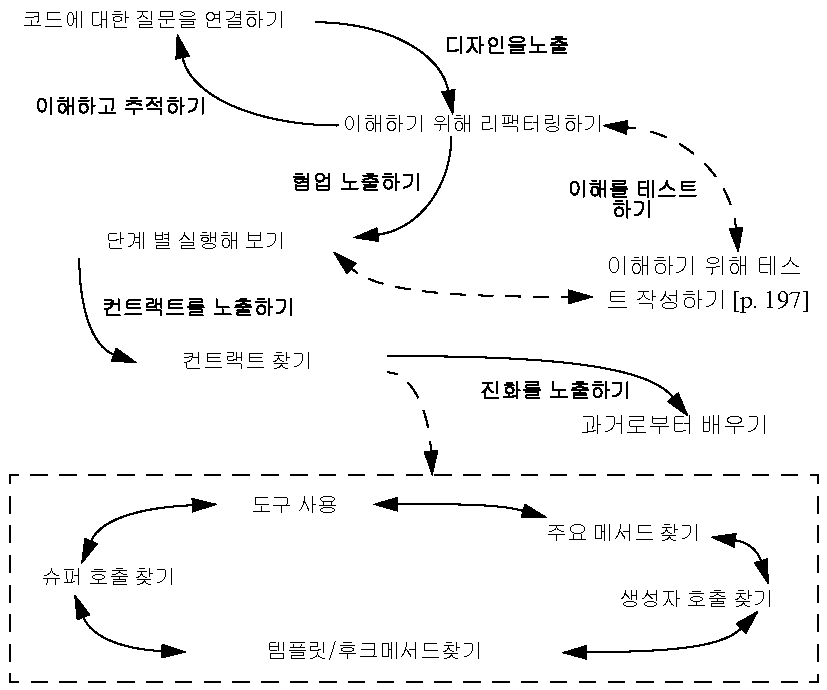
\includegraphics[width=\textwidth]{oldDetailedModelMap.pdf}
\caption{\charef{상세 모델 캡춰하기}{DetailedModelCapture}의 패턴은 소프트웨어 시스템의 설계를 노출하고 이해도를 추적하는 데 도움이 된다.}
\figlabel{DetailedModelMap}
\end{center}
\end{figure}

\figref{DetailedModelMap}은 패턴 간의 몇 가지 가능한 관계를 제안한다. 패턴 중 가장 기본적이고 적용하기 가장 쉬운 패턴은 \patref{코드에 대한 질문을 연결하기}{TieCodeAndQuestions}이다. 소스 코드를 살펴보면서 주석, 질문, 가설 및 수행 가능한 작업을 추적하여 소스 코드에 직접 \emph{주석이 적용되는 지점에} 주석을 달아 놓자. 이 패턴은 이 클러스터의 다른 패턴과 잘 작동하며 리엔지니어링 프로젝트 전반에 걸쳐 생산적으로 적용될 수 있다.

\patref{이해하기 위해 리팩터링하기}{RefactorToUnderstand}는 암호화된 코드의 설계를 노출하는 데 도움이 된다. 이 패턴의 의도는 코드 베이스 자체를 개선하는 것이 아니라 이해력을 향상시키는 데 있다는 점을 이해하는 것이 중요하다. 리팩터링의 결과를 유지하기로 결정할 수도 있지만, 이 시점에서 이것이 목표가 되어서는 안 된다. 리팩터링은 코드와 관련된 다양한 가설을 테스트하기 위한 실험으로 간주해야 한다. 

소스 코드는 클래스 계층 구조에 대한 매우 정적인 보기만 제공하므로 \patref{단계 별 실행해 보기}{StepThroughTheExecution}을 사용하여 어떤 객체가 인스턴스화되고 런타임에 어떻게 상호 작용하는지 알아보는 것이 유용하다.

시스템에서 클래스의 인터페이스를 추출하는 것은 매우 쉽지만, 이러한 인터페이스가 어떻게 사용될 수 있는지 또는 어떻게 사용해야 하는지에 대해 많은 것을 알려주지는 않는다. 실제로 필요한 것은 각 클래스에서 지원하는 \patref{컨트랙트 찾기}{LookForTheContracts}를 수행하는 것이다. 컨트랙트는 어떤 클라이언트-공급자 관계가 존재하는지, 클래스의 공용 인터페이스가 그 관계를 어떻게 지원하는지 알려준다. 관용적 코딩 관행과 디자인 패턴은 일반적으로 이러한 계약을 직접적인 방식으로 표현하므로 이를 인식할 수 있도록 스스로 훈련해야 한다.

마지막으로, 소스 코드에서 다양한 디자인 산출물을 추출할 수는 있지만 시스템이 어떻게 그런 식으로 진화했는지에 대한 통찰력을 반드시 얻을 수 있는 것은 아니다. 특히 특정 설계 결정이 정말 정당한 것인지, 아니면 자의적인 것인지 궁금할 수 있으며, 설계의 일부가 얼마나 안정적인지 궁금할 수 있다. 코드 베이스의 여러 버전을 비교하고 기능이 제거되거나 리팩터링된 부분을 집중적으로 살펴봄으로써 과거로부터 \patref{과거로부터 배우기}{LearnFromThePast}를 할 수 있다.

\subsection*{다음 단계}

이제 시스템 일부의 세부 사항을 마스터했으니 \charef{테스트라는 생명 보험}{TestsYourLifeInsurance}의 패턴을 적용하여 실제 리엔지니어링을 준비할 때이다. 특히 \patref{이해하기 위해 리팩터링하기}{RefactorToUnderstand}와 같은 패턴은 실험에 자신감을 줄 수 있으므로 \patpgref{이해하기 위해 테스트 작성하기}{WriteTestsToUnderstand}와 같은 패턴을 사용하는 것이 좋다. 또한 \patref{단계 별 실행해 보기}{StepThroughTheExecution}, \patref{컨트랙트 찾기}{LookForTheContracts}, \patref{과거로부터 배우기}{LearnFromThePast} 같은 패턴은 어떤 구성 요소가 어떤 기능을 구현하는지 파악하는 데 도움이 된다. 이 지식은 \patpgref{구현이 아닌 인터페이스 테스트하기}{TestTheInterfaceNotTheImplementation} 및 \patpgref{비즈니스 규칙을 테스트로 기록하기}{RecordBusinessRulesAsTests}에 사용해야 한다.


%=================================================================
%:PATTERN -- {Tie Code and Questions}
\pattern{코드에 대한 질문을 연결하기}{TieCodeAndQuestions}

\intent{리엔지니어링 활동과 관련된 질문과 답변을 소스 파일에 직접 저장하여 코드와 동기화한다.}

\subsection*{문제}

코드와 그에 대해 궁금한 점을 어떻게 \emph{이해하고 추적하고}, 향후 코드가 발전하는 동안 이러한 \emph{코멘트를 코드와 동기화하고}, 다른 팀원들과 \emph{공유하는가?} 

\emph{이 문제는 다음과 같은 이유로 어렵다.}

\begin{bulletlist}
\item 분석 중인 시스템에 대해 알고 있는 것과 모르는 것을 작성하는 것은 지루하고 시간이 많이 걸린다.

\item 시스템을 이해하는 것은 움직이는 과녁과 같아서 문서화를 최신 상태를 유지하기가 어렵습니다.

\item 질문과 인사이트가 떠오르는 즉시 기록하지 않으면 이를 추적할 수 없다.

\item 지식을 팀과 공유하여 그 가치를 극대화하고 싶다.

\item 로그 파일, 게시판 또는 이메일 배포 목록에 질문과 답변을 기록하면 팀 내에서 지식을 전파하는 데 편리하고 팀이 이해한 내용을 편리하게 검색할 수 있지만 코드 조각을 볼 때 어떤 질문과 답변이 해당 코드와 관련이 있는지 알기 어려울 수 있다.
\end{bulletlist}

\emph{그러나 이 문제를 해결할 수 있는 이유는 다음과 같다.}

\begin{bulletlist}
\item 코드에 에너테이션(annotation)을 달 수 있으므로 참조하는 코드 요소에 물리적으로 가깝게 이해한 내용을 기록할 수 있다.
\end{bulletlist}

\subsection*{솔루션}

코드를 작업하는 동안 직면하고 있는 질문에 직접 즉시 에너테이션을 달아 보자. 

원칙적으로 코드에 에너테이션을 다는 방법에는 두 가지가 있다.

\begin{bulletlist}
\item \emph{주석 기반 에너테이션.}
이 접근 방식은 프로그래밍 언어의 주석 규칙을 사용하므로 텍스트 중심 환경에 더 적합하다. 일반 주석과 에너테이션을 구분하기 위해 몇 가지 규칙이 필요하다.

% 코드는 한글로 넣으면 에러가 난다.
\begin{code}
/*  #to: John #by: SD #on: 3/12/99 *****
    Screws up when we have nested I Fs. */
\end{code}
그런 다음 프로그램 환경의 일부인 기본 도구를 사용하여 주석을 검색하고 수정할 수 있다. 약간의 추가 노력으로 모든 주석 기반 에너테이션을 쿼리, 추출 및 교차 색인하는 도구를 쉽게 만들 수 있다.

\item \emph{메서드 기반 에너테이션.}
이 접근 방식은 오늘날의 많은 프로그래밍 환경에서 제공하는 기능인 특정 메서드를 호출하는 메서드를 쿼리할 수 있는 가능성을 활용한다. 이 아이디어는 몇 개의 문자열을 인수로 받아들이고 메서드 본문이 비어 있는 전역 메서드를 선언하는 것입니다. 특정 코드에 주석을 달고 싶을 때마다 해당 메서드를 호출하여 주석을 매개변수로 전달하면 된다.

% 코드는 한글로 넣으면 에러가 난다.
\begin{code}
this.annotateCode("#to: John #by: SD #on: 3/12/99",
    "Screws up when we have nested I Fs.");
\end{code}
그런 다음 프로그래밍 환경의 쿼리 및 탐색 기능을 사용하여 이 특수 메서드가 호출되는 위치, 즉 주석이 발생하는 위치를 식별할 수 있다. 대부분의 프로그래밍 환경은 작은 스크립트를 통해 확장할 수 있으며, 이 경우 모든 주석에 대한 보고서를 생성하는 도구를 개발할 수 있다.

코드를 덜 변경할수록 오류가 발생할 가능성이 줄어든다는 점에 알아두자. 따라서 주석 기반 버전이 메서드 기반 버전보다 더 안전하다.
\end{bulletlist}

\subsubsection*{힌트}

\begin{bulletlist}
\item 에너테이션은 참조하는 코드에 \emph{가능한 한 가깝게} 기록하자.

\item 에너테이션은 나중에 참조할 수 있도록 기록하려는 코드에 대한 \emph{질문}, \emph{가설}, \emph{``할 일'' 목록} 또는 단순히 \emph{관찰 사항}이 될 수 있다.

\item 규칙을 사용해 \emph{에너테이션을 구별하자}. 예를 들어 팀 맥락에서는 주석을 작성한 개발자의 이니셜과 주석을 입력한 날짜를 포함하자. 이렇게 하면 쉽게 쿼리할 수 있다.

\item \emph{회사 관행을 따르자.} 댓글이 영어가 아닌 다른 언어로 작성된 경우 가능한 경우 계속 진행하자. 그러나 선택의 여지가 있다면 소스 코드가 작성된 언어(대부분의 경우 영어)와 다른 언어로 주석을 작성하지 않도록 하자. 그렇지 않으면 다른 컨텍스트를 만들어 독자가 그 사이에서 전환해야 한다. 

\item 질문 중 하나에 대한 \emph{답변}을 발견하면 향후 독자를 위해 주석을 \emph{즉시 업데이트}하거나 더 이상 관련이 없는 질문은 간단히 \emph{삭제}하자.
\end{bulletlist}

\subsection*{트레이드오프}

\subsubsection*{장점}

\begin{bulletlist}
\item \emph{자연적인 동기화.} 코드와 주석을 물리적으로 가깝게 유지하면 코드와 주석이 동기화될 확률이 높아진다. 코드를 수정하는 동안 자연스럽게 에너테이션을 수정하거나 더 이상 사용되지 않는 경우 에너테이션을 제거할 수 있다.

\item \emph{팀 커뮤니케이션 개선.} \patref{코드에 대한 질문을 연결하기}{TieCodeAndQuestions}를 사용하면 팀원이 별도의 커뮤니케이션 채널(이메일, 게시판, $\cdots$)을 열지 않아도 된다. 팀원들은 어떻게든 자신이 작업하는 코드를 읽어야 하므로 코드를 커뮤니케이션 채널로 사용하여 다중화할 수 있다.

\item \emph{컨텍스트 설명 최소화.} 코드에 주석을 달면 즉시 컨텍스트를 파악할 수 있다. 이렇게 하면 질문의 맥락을 설명할 필요성을 최소화하고 질문과 주석을 문서화하는 데 드는 노력을 줄일 수 있다.
\end{bulletlist}

\subsubsection*{단점}

\begin{bulletlist}
\item \emph{본질적으로 수동적.} 입력한 질문이 반드시 누구에게 전달되는 것은 아니며, 전달되더라도 수신자가 제때 읽거나 답변할지 확신할 수 없다. 주석을 수집하고 적절한 사람에게 알리려면 추가 도구가 필요할 수도 있다.


\item \emph{프로세스 비호환성.} 많은 회사가 계층적 보고 구조를 중심으로 조직되어 있다. 이러한 조직에서는 \patref{코드에 대한 질문을 연결하기}{TieCodeAndQuestions}가 정상적인 커뮤니케이션 채널을 우회하기 때문에 거부될 수 있다. 또한 일부 기업 관행에서는 프로그래머가 코드로 할 수 있는 작업에 강력한 제약을 가하기 때문에 이 패턴을 사용할 경우 잠재력이 제한될 수 있다. 예를 들어, 주석이 더 이상 사용되지 않을 때 제거할 수 없다면 너무 많은 노이즈가 발생하여 유용하지 않게 된다.
\end{bulletlist}

\subsubsection*{어려움}

\begin{bulletlist}
\item \emph{적합한 세분성 찾기.} 모든 종류의 주석과 마찬가지로 적절한 양의 세부 정보를 소개하는 데 주의를 기울여야 한다. 간결하거나 난해한 주석은 금방 가치를 잃고, 장황한 주석은 독자의 주의를 코드 자체로부터 분산시킬 수 있다.

\item \emph{프로그래머가 주석을 작성하도록 동기 부여하기.} 프로그래머는 일반적으로 주석이나 문서를 작성하는 것을 좋아하지 않는다. 동기를 부여하는 한 가지 방법은 코드 리뷰나 상태 회의 중에 주석을 사용하는 것이다. 이렇게 하면 주석이 즉각적인 이점을 제공한다.

\item \emph{답변의 품질.}
다른 종류의 문서와 마찬가지로 잘못된 답변이 제공될 수 있다. 이러한 상황에 대처하는 한 가지 방법은 팀 내에서 주석을 정기적으로 검토하는 것이다.

\item \emph{에너테이션 제거하기.}
어떤 경우에는 주석을 제거하고 싶을 수도 있다. 예를 들어, 고객에게 ``깨끗한'' 버전의 소스 코드를 제공해야 하거나 컴파일러가 빈 메서드 바디의 호출을 제거할 만큼 똑똑하지 않은 경우이다. 이 경우 에너테이션을 필터링할 수 있는 적절한 도구가 있는지 확인하자.
\end{bulletlist}

\subsection*{근거}

이 패턴의 뿌리는 \emphind{문학적 프로그래밍(literate programming)}에 있다. \cite{Reen89a}\cite{Knut92a}. 문학적 프로그램은 프로그램 텍스트와 주석 사이의 일반적인 관계를 뒤집어 실행 코드가 문서 안에 포함되는 것이 아니라 그 반대가 된다. 문학적 프로그래밍은 코드와 문서를 물리적으로 가깝게 유지하는 데 중점을 둔다. 물리적으로 가까우면 코드와 문서를 동기화하는 데 드는 노력이 줄어든다.

\subsection*{알려진 용도}

\emph{주석 기반 에너테이션.}
다양한 프로그래밍 환경에서는 코드 내 에너테이션 관리를 암시적으로 지원한다. 예를 들어, Emacs에는 e-tag라는 도구가 내장되어 있어 \cite{Came96a} 파일 집합의 상호 참조 데이터베이스를 쉽게 생성할 수 있다. 반면에 \ind{Eiffel} 환경에서는 댓글(및 코드)에 다양한 수준의 가시성을 할당할 수 있다. 에너테이션에 비공개 범위를 지정하면 에너테이션을 쉽게 분리하면서도 외부에 표시되지 않도록 할 수 있다.

벨기에의 멀티미디어 분야 회사인 \ind{MediaGeniX}는 체계적인 코드 태깅 메커니즘을 사용해 변경 사항에 대한 정보를 기록했다. 프로그래밍 환경은 코드가 변경될 때마다 코드 변경 동기(버그 수정, 변경 요청, 새 릴리스), 개발자 이름, 수정 시간을 설명하는 태그가 자동으로 주석이 달리는 방식으로 변경되었다. 마지막 태그만 코드에 보관되지만 구성 관리 시스템을 통해 이전 태그와 변경 사항을 검사할 수 있다. 이 태그에는 개발자가 원하는 내용을 작성할 수 있는 자유 필드도 포함되어 있어 질문과 답변에 자주 사용된다. 

\noindent
\emph{메서드 기반 에너테이션.}
\ind{Squeak} 개발팀 \cite{Inga97a}는 이 기술을 질문을 추적하기 위한 것이 아니라 오픈소스 개발 프로젝트에서 커뮤니케이션을 원활하게 하기 위한 수단으로 사용했다. 이 팀에서는 메서드 플래그를 호출하는 방식으로 코멘트를 도입했는데, 이는 \lct{Object} 클래스에 정의되어 있다. 개발자는 flag: 메시지를 보낸 모든 발신자를 쿼리하여 주석을 찾을 수 있다. 또한 이 메서드는 심볼을 인자로 받도록 정의되어 있다. 이를 통해 예를 들어 \ct{#noteForJohn} 기호로 플래그가 지정된 모든 에너테이션을 보다 구체적으로 검색할 수 있다.

% 코드에는 한글을 넣을 수 없다.
\begin{code}
Object>>flag: aSymbol
	"Send this message, with a relevant symbol as argument, to flag
	a message for subsequent retrieval. For example, you might put 
	the following line in a number of messages:
		self flag: #returnHereUrgently
	Then, to retrieve all such messages, browse all senders of
	#returnHereUrgently."
\end{code}

\begin{figure}
\begin{center}
\includegraphics[width=\textwidth]{DetailedModelAllSenders}
\caption{Squeak에서 메시지의 모든 발신자 찾기.}
\figlabel{DetailedModelAllSenders}
\end{center}
\end{figure}

\figref{DetailedModelAllSenders}는 Squeak2.7 환경에서 플래그: 메시지의 모든 발신자를 위쪽 창에 표시한다. 그러면 아래쪽 창에 flag: 메서드 호출이 포함된 \lct{removeEmptyRows} 메서드의 코드가 강조 표시되어 표시된다. flag: 메시지는 인자 \lct{\#noteToJohn}과 함께 전송된다. 에너테이션의 실제 내용은 코멘트로 이어진다. 

\subsection*{관련된 패턴}

\patref{코드에 대한 질문을 연결하기}{TieCodeAndQuestions}는 \patref{이해하기 위해 리팩터링하기}{RefactorToUnderstand}와 함께 잘 작동헌다. 코드의 의문점은 종종 리팩터링을 통해 해결될 수 있다. 반대로 \patref{이해하기 위해 리팩터링하기}{RefactorToUnderstand}를 사용하면 새로운 질문이 제기되고 에너테이션으로 입력할 수 있다.

%=================================================================
%:PATTERN -- {Refactor to Understand}
\pattern{이해하기 위해 리팩터링하기}{RefactorToUnderstand}

\intent{소프트웨어 시스템의 작동 방식에 대한 이해를 검증하고 반영하기 위해 소프트웨어 시스템의 일부를 반복적으로 리팩터링한다.}

\subsection*{문제}

암호화된 것 같은 코드를 어떻게 이해할 수 있는가?

\emph{이 문제는 다음과 같은 이유로 어렵다.}

\begin{bulletlist}
\item 암호화된 것같은 코드는 읽기 어렵기 때문에 이해하기 어렵다.

\item 코드가 어떻게 작동하는지 어느 정도는 알 수 있지만 코드가 여러분의 아이디어를 반영하지 않아 확인하기가 어렵다.
\end{bulletlist}

\emph{그러나 이 문제를 해결할 수 있는 이유는 다음과 같다.}

\begin{bulletlist}
\item 코드 조각이 \emph{상대적으로 작고} 경계가 명확하게 정의되어 있다.

\item 개발 도구에서 \emph{빠르게 편집-컴파일 반복하기}를 허용하므로 약간의 변경을 수행하고 소스 코드를 컴파일할 수 있는지 또는 테스트가 계속 실행되는지 확인할 수 있다.

\item 소스 코드 엔티티 간의 종속성(예: 어떤 메서드가 주어진 작업을 호출하는지, 어떤 메서드가 주어진 속성에 액세스하는지 등)을 쿼리할 수 있는 \emph{소스 코드 브라우저}가 있으므로 그 목적을 유추할 수 있다.
\end{bulletlist}

\subsection*{솔루션}

반복적으로 코드의 이름을 바꾸고 리팩터링하여 의미 있는 이름을 도입하고 코드의 구조가 시스템이 실제로 수행하는 작업을 반영하는지 확인한다. 변경할 때마다 레그레션 테스트(regression tests)가 가능한 경우 이를 실행하고, 그렇지 않은 경우 자주 컴파일하여 변경 사항이 합당한지 확인한다. 코드를 리팩토링한 후 코드를 어떻게 처리할지 결정하자.

\subsubsection*{힌트}

여기서 가장 중요한 목표는 코드를 개선하는 것이 아니라 시스템을 이해하는 것이다. 따라서 코드에 대한 변경 사항은 코드에 대한 이해를 테스트하기 위한 ``실험(experiments)''으로 취급해야 한다. 따라서 시작하기 전에 코드의 복사본을 만들어야 한다. 코드를 리팩터링한 후에는 변경한 내용을 릴리스할 수도 있지만, 미리 결정하고 싶지는 않을 것이다. 리팩터링 실험을 통해 실제로 코드가 개선될 수도 있지만, 아직 코드를 이해하지 못하기 때문에 일을 엉망으로 만들 가능성도 똑같이 높다. 이 단계에서는 크게 중요하지 않다. 첫 경험을 하고 나면 리팩터링을 제대로 할 수 있는 더 나은 위치에 서게 될 것이다. 

변경 사항이 아무것도 깨뜨리지 않았는지 확인할 수 있는 테스트가 없다면 리팩터링을 제대로 수행하기 어렵다. 적절한 테스트가 없다면 리팩터링 실험 결과를 보관하는 것을 심각하게 고려하지 않아야 한다. 그러나 \patref{이해하기 위해 테스트 작성하기}{WriteTestsToUnderstand}를 \patref{이해하기 위해 리팩터링하기}{RefactorToUnderstand}와 함께 적용하는 것을 고려하자. 

코드에서 설계 결정을 보다 명확하게 할 수 있는 리팩터링 작업을 선택해야 한다. 이 반복적인 재구조화 중에 적용되는 일반적인 리팩터링은 \patpgref{속성 이름 바꾸기}{RenameAttribute}, \patpgref{메서드 이름 바꾸기}{RenameMethod} 및 \patpgref{메서드 추출하기}{ExtractMethod}이다.

다음 가이드라인은 코드의 가독성을 개선하기 위해 이러한 리팩터링을 적용하는 위치와 방법을 찾는 데 도움이 될 것이다. 이러한 가이드라인 중 다수는 Smalltalk 프로그래밍 \cite{Beck97a}에서 좋은 표준 관행으로 간주된다. 그러나 다른 프로그래밍 언어에도 동일하게 적용된다. 어떤 순서로든 적용될 수 있으며, 각 지침은 다른 지침을 이해하는 데 도움이 된다.

\begin{bulletlist}
\item \emph{역할(role)을 전달하기 위해 속성(attribute)의 이름을 바꾼다.}
암호화된 겉 같은 이름을 가진 속성에 집중하자. 속성의 역할을 파악하려면 모든 속성 액세스(접근자 메서드 호출 포함)를 살펴보자. 그런 다음 역할에 따라 속성(attribute)와 해당 접근자(accessor)의 이름을 바꾸고 모든 참조를 업데이트하고 시스템을 다시 컴파일하자.

\item \emph{의도를 전달하기 위해 메서드 이름 바꾸기.}
의도를 드러내는 이름이 없는 메서드의 의도를 검색하려면 모든 호출과 속성 사용을 조사하고 메서드의 책임을 추론한다. 그런 다음 의도에 따라 메서드의 이름을 바꾸고 모든 호출을 업데이트한 후 시스템을 다시 컴파일한다.

\item \emph{목적(purpose)을 전달하기 위해 클래스 이름 바꾸기.}
이름이 불분명한 클래스의 목적을 파악하려면 해당 클래스의 클라이언트를 조사하여 누가 해당 연산을 호출하는지 또는 누가 해당 클래스의 인스턴스를 생성하는지 조사하자. 그런 다음 목적에 따라 클래스 이름을 변경하고 모든 참조를 업데이트한 후 시스템을 다시 컴파일하자.

\item \emph{중복된 코드 제거.}
중복된 코드를 발견하면 한 곳으로 리팩터링하자. 이렇게 하면 리팩토링 전에는 알아차리지 못했을 사소한 차이점을 식별하고 미묘한 디자인 문제를 드러낼 수 있다. 

\item \emph{조건 분기를 메서드로 대체.}
큰 가지가 있는 조건이 있는 경우 해당 가지를 새로운 (프라이빗) 메서드(private method)로 추출하자. 이러한 메서드의 이름을 지정하려면 조건을 충분히 이해하여 의도를 드러내는 이름을 선택할 수 있을 때까지 조건을 연구하자.

\item \emph{메서드 본문을 일관된 추상화 수준으로 리팩터링.}
코드 블록을 구분하는 주석이 있는 긴 메서드 본문은 단일 메서드 본문의 모든 문이 동일한 수준의 추상화를 가져야 한다는 경험 법칙을 위반한다. 분리된 각 코드 블록에 새로운 (프라이빗) 메서드(private method)를 도입하여 이러한 코드를 리팩터링하고, 주석에 기록된 의도를 따라 메서드 이름을 지정하자.
\end{bulletlist}

\subsection*{트레이드오프}

\subsubsection*{장점}

\begin{bulletlist}
\item \emph{디자인 노출.}
리팩토링 프로세스를 통해 코드에 대한 이해도가 향상될 뿐만 아니라 코드 구조에 대한 이해도도 명확해진다. 이렇게 하면 \patref{코드에 대한 질문을 연결하기}{TieCodeAndQuestions} 또는 \patpgref{이해하기 위해 테스트 작성하기}{WriteTestsToUnderstand}를 통해 이해도를 더욱 쉽게 문서화할 수 있다.

\item \emph{증가하는 유효성 검사.}
일반적으로 이해는 단일 계시의 일부로 발생하는 것이 아니라 이전 이해가 다음 반복의 기반이 되는 반복적인 과정의 결과로 발생한다. \patref{이해를 위해 리팩터링하기}{RefactorToUnderstand}는 작은 단계와 빈번한 검증(테스트를 실행하거나 자주 컴파일하여)을 강조하기 때문에 이러한 접근 방식을 권장한다.
\end{bulletlist}

\subsubsection*{단점}

\begin{bulletlist}
\item \emph{오류 발생 리스크.}
코드를 적게 변경할수록 오류가 발생할 가능성이 줄어든다. 작은 리팩터링은 동작을 보존해야 하지만, 간단한 리팩터링이라도 코드가 깨지지 않는지 확인하는 것은 쉽지 않을 수 있다. 적절한 레그레션 테스트가 마련되어 있지 않은 경우 변경 사항을 도입하는 것이 위험하거나 필요한 테스트를 개발하는 데 비용이 많이 들 수 있다. 이러한 이유로 소프트웨어의 작업 복사본에서만 \patref{이해하기 위해 리팩터링하기}{RefactorToUnderstand}를 시도하는 것이 중요하다.
\end{bulletlist}

\subsubsection*{어려움}

\begin{bulletlist}
\item \emph{도구 지원.}
수동으로 코드를 리팩토링하는 것은 지루하고 위험할 수 있다 \cite{Fowl99a}. \ind{리팩토링 브라우저}\emph{(Refactoring Browser)}와 같은 다양한 도구가 있다. \cite{Robe97a}와 같은 다양한 도구는 리팩터링 작업을 크게 간소화하며, 특히 \patref{메서드 추출하기}{ExtractMethod}와 같이 사소하지 않은 리팩터링을 적용하는 데 도움이 된다.

\item \emph{변경 수락.}
다른 사람의 코드를 리팩토링하는 것은 자신의 코드를 리팩토링하는 것보다 훨씬 더 어려울 수 있다. 많은 회사에서 코드 소유권 문화가 강하기 때문에 다른 사람의 코드를 개선하는 것은 종종 모욕으로 간주된다. 이것이 바로 리팩터링된 버전을 반드시 다른 팀원에게 공개해서는 안 되는 이유 중 하나이다.

\item \emph{멈춤 시기.}
문제를 발견했을 때 코드 변경을 중단하기 어려운 경우가 많다. 여기서 여러분의 일차적인 목표는 시스템을 이해하는 것임을 기억하자. 그 목표를 달성했다면 이제 멈춰야 할 때이다. 
\end{bulletlist}

\subsection*{알려진 용도}

\index{로버트, 돈}
\index{브랜트, 존}
돈 로버츠와 존 브랜트는 ESUG '97과 Smalltalk Solutions '97에서 \emph{리팩터링 브라우저}를 시연하는 동안 \patref{이해하기 위해 리팩터링하기}{RefactorToUnderstand}라는 용어를 만들었다. 그들은 코드의 이름을 바꾸고 리팩토링하여 알고리즘을 점차적으로 이해하는 과정을 보여주었다. 이후 이 패턴을 반복하는 동안 코드가 서서히 이해되기 시작했고 디자인이 점차 코드에 명시적으로 드러나기 시작했다. 

저희는 이 패턴을 \ind{FAMOOS} 사례 연구에 직접 적용했다. 우리는 약 3000줄의 \ind{C++}로 이루어진 하나의 메서드를 이해해야 했는데, 이 메서드는 중첩된 조건 명령을 가졌다. 먼저 리프 조건 분기를 메서드로 대체하면서 중첩 구조를 점차적으로 파악해 나갔다. 몇 번의 반복 끝에 이 메서드가 실제로 작은 명령어에 대한 완전한 파서를 구현하고 있다는 것을 발견했다. 

\index{스니드, 해리}
해리 스니드는 모든 goto 문을 제거하여 대규모 \ind{Cobol} 프로그램을 리팩터링한 여러 리엔지니어링 프로젝트에 대해 리포트를 만들었다. 그러나 나중에 개발자들이 그의 변경 사항을 거부했기 때문에 \cite{Snee99a}를 다시 goto문을 도입할 수밖에 없었다.

\subsection*{관련된 패턴}

``\ind{가구 배치}''\emph{(Arranging the Furniture)} \cite{Tayl00a}는 새 프로젝트에 새로 들어온 사람이 편안하게 시작할 수 있도록 도와주는 패턴이다. 이 패턴의 해결책은 ``코드를 깔끔하게 정리하여 `적응'하도록 도입하는 사람이 유도해야 한다''이다. 

\subsection*{다음 단계}

\patref{이해하기 위해 리팩터링하기}{RefactorToUnderstand}는 \patref{코드에 대한 질문을 연결하기}{TieCodeAndQuestions}와 함께 잘 작동한다. 리팩터링은 단순히 코드에 주석을 다는 것보다 구현하는 데 비용이 많이 들기 때문에 먼저 주석을 다는 작업을 한 다음 리팩터링하자. 또한 리팩터링할 때 \patpgref{이해할 수 있는 테스트 작성하기}{WriteTestsToUnderstand}를 고려하자. 테스트는 소프트웨어 산출물의 작동 방식에 대한 이해를 문서화하고 리팩터링은 디자인을 노출하는 데 도움이 되므로 이 두 가지 활동은 서로를 강화한다. 또한 테스트는 리팩터링으로 인해 문제가 발생하지 않았는지 확인하는 데 도움이 된다.

\patref{이해를 위해 리팩터링하기}{RefactorToUnderstand}를 완료했다면, 변경 사항을 어떻게 처리할지 결정해야 한다. 실험 코드를 폐기하는 경우 \patref{코드에 대한 질문 연결하기}{TieCodeAndQuestions}를 적용하여 습득한 지식으로 코드 베이스에 주석을 달아야 한다.

%=================================================================
%:PATTERN -- {Step Through the Execution}
\pattern{단계 별 실행해 보기}{StepThroughTheExecution}


\intent{시스템의 객체들이 어떻게 협업하는지 \ind{디버거}에서 예제를 단계별로 실행해 보고 이해한다.}

\subsection*{문제}

런타임에 어떤 객체가 인스턴스화되고 어떻게 협업하는지 어떻게 알 수 있는가?

\emph{이 문제는 다음과 같은 이유로 어렵다.}

\begin{bulletlist}
\item 소스 코드는 런타임에 인스턴스화된 객체와 객체 간 상호 작용 방식이 아닌 클래스 계층 구조를 노출한다.

\item 협업은 일반적으로 코드를 통해 분산되어 있다. 시스템에서 어떤 클래스와 메서드가 정의되어 있는지 쉽게 확인할 수 있지만, 소스 코드만으로는 어떤 이벤트 시퀀스로 인해 객체가 생성되거나 메서드가 호출되는지 알기 어려울 수 있다.

\item 다형성(polymorphism)이 있는 경우 어떤 객체가 어떤 서비스 제공자의 클라이언트인지 구분하기가 특히 어려울 수 있다. 한 객체가 다른 객체가 제공하는 특정 인터페이스를 사용한다고 해서 전자가 실제로 후자의 클라이언트라는 의미는 아니다.

\item 코드를 읽는다고 해서 어떤 구체적인 시나리오가 발생할 수 있는지 알 수 없다. 실제 실행 흐름은 모든 참여 객체의 내부 상태에 따라 달라지며 이는 소스 코드에서 직접 유추할 수 없다.

\item 소스 코드는 어떤 객체가 수명이 긴지, 어떤 객체가 일시적인지(즉, 단일 메서드의 실행에 국한되는지) 알려주지 않는다.
\end{bulletlist}

\emph{그러나 이 문제를 해결할 수 있는 이유는 다음과 같다.}

\begin{bulletlist}
\item 몇 가지 일반적인 사용 시나리오를 알고 있다.

\item 디버거 내에서 코드를 실행할 수 있다.

\item 시스템의 일부에 주의를 집중하고 있다.
\end{bulletlist}

\subsection*{솔루션}

각 시나리오를 실행하고 디버거를 사용하여 코드를 단계별로 살펴보자. 어떤 객체가 협업하고 어떻게 인스턴스화되는지 관찰하자. 그런 다음, 이러한 관찰을 일반화하고 나중에 참조할 수 있도록 \patref{코드에 대한 질문을 연결하기}{TieCodeAndQuestions} 및 \patpgref{비즈니스 규칙을 테스트로 기록하기}{RecordBusinessRulesAsTests}를 사용하여 알게된 지식을 기록해 두자.

\subsubsection*{힌트}

실행 중인 시스템의 모든 문을 일일이 살펴보기에는 시간이 너무 많이 걸린다. 여기서는 이해하기 어려운 시스템의 특정 측면에 초점을 맞추고 있다고 가정한다.

\begin{bulletlist}
\item 시스템이 관심 있는 코드에 들어갈 때 실행을 중단하도록 \emph{브레이크포인트(breakpoint)}를 설정한다.

\item 개체의 \emph{내부 상태(internal state)}를 변경하여 대체 실행 경로가 어떻게 트리거되는지 확인한다.

\item 현재 실행 스택에 있는 \emph{메서드 다시 시작(restart a method)}을 사용하여 유사한 시나리오를 빠르게 확인할 수 있다.
\end{bulletlist}

\subsection*{트레이드오프}

\subsubsection*{장점}

\begin{bulletlist}
\item \emph{현실적 뷰.}
실행 중인 프로그램을 단계별로 살펴보면 시나리오가 어떻게 전개되는지 정확하게 파악할 수 있다. 또한 관련된 객체의 내부 상태를 검사하고, 새로운 객체가 어떻게 생성되는지 확인하고, 어떤 상황에서 어떤 객체가 협업하는지 관찰할 수 있다.

\item \emph{복잡성 다루기.}
소규모로 소스 코드를 분석하여 객체 협업을 유추할 수 있다. 예를 들어 슬라이싱 도구는 소스 코드의 어떤 문이 주어진 변수의 영향을 받는지 알려줄 수 있다. 그러나 크고 복잡한 시스템의 경우 가능성과 상호 작용의 수가 너무 많다. 따라서 객체가 어떻게 협업하는지 알아내는 유일한 합리적인 방법은 실행 추적을 연구하는 것이다.
\end{bulletlist}

\subsubsection*{단점}

\begin{bulletlist}
\item \emph{시나리오 기반.}
제한된 시나리오 집합으로 제한해야 하므로 관찰된 개체-협업은 반드시 불완전할 수밖에 없다. 물론 대표 시나리오를 선택하기 위해 최선을 다해야 한다. 안타깝게도 이러한 선택은 다시 원점으로 돌아가게 된다. 왜냐하면 대표적인 시나리오 집합이 있는지 확인하는 유일한 방법은 가능한 모든 개체 협업을 포함하는지 확인하는 것이기 때문이다.

\item \emph{제한된 적용가능성(applicability).}
시간이 중요한 역할을 하는 시스템의 경우 실행을 단계별로 진행하면 시스템의 동작을 비현실적으로 파악할 수 있다. 더 나쁜 것은 동시 또는 분산 시스템의 경우 동시 코드를 단계별로 살펴본다는 사실만으로도 시스템 실행 자체가 교란될 수 있다는 점입이다. 따라서 양자 입자의 정확한 위치를 결정하면 해당 입자에 대한 다른 속성이 불확실해지는 하이젠베르크의 불확실성 실험(Heisenberg's uncertainty experiments)과 같은 효과를 얻을 수 있다.
\end{bulletlist}

\subsubsection*{어려움}

\begin{bulletlist}
\item \emph{도구 의존성.}
\patref{단계별 실행해 보기}{StepThroughTheExecution}를 위한 좋은 디버거가 있어야 한다. 중단점을 동적으로 설정하고 제거할 수 있어야 할 뿐만 아니라 관련된 객체의 상태를 검사할 수 있는 수단도 제공해야 한다. 또한 대체 경로를 쉽게 확인할 수 있도록 디버거는 객체의 내부 상태를 변경하거나 현재 실행 스택에 있는 메서드를 다시 시작할 수도 있어야 한다.
\end{bulletlist}

\subsection*{다음 단계}

\patref{단계별 실행해 보기}{StepThroughTheExecution}(아마도 \patpgref{데모 중 인터뷰하기}{InterviewDuringDemo}에서 유추 가능)를 수행하려면 구체적인 시나리오가 필요하다. 이러한 시나리오를 테스트 케이스로 인코딩하는 것을 고려해 보자. 그런 다음 \patref{이해하기 위해 테스트 작성하기}{WriteTestsToUnderstand}을 반복적으로 수행하면 협업 객체의 상태에 대한 통찰력을 구체적인 테스트로 공식화할 수 있으므로 \patpgref{이해하기 위해 테스트 작성하기}{WriteTestsToUnderstand}을 반복적으로 수행할 수 있다.

\patref{단계 별 실행해 보기}{StepThroughTheExecution}을 사용할 때 협업하는 개체가 서로의 인터페이스를 사용하는 방식을 계속 주시하는 것이 좋다. 그 후에는 \patref{컨트랙트 찾기}{LookForTheContracts}에 습득한 지식을 활용할 수 있다.

%=================================================================
%:PATTERN -- {Look for the Contracts}
\pattern{컨트랙트 찾기}{LookForTheContracts}

\intent{클라이언트가 현재 사용하는 방식을 연구하여 클래스 인터페이스(class interface)의 적절한 사용법을 추론한다.}

\subsection*{문제}

클래스가 어떤 컨트랙트(contracts)를 지원하는지 어떻게 결정하는가? 즉, 클래스가 의도한 대로 작동하기 위해 클라이언트 클래스에서 무엇을 기대하는지 어떻게 알 수 있을까?

\emph{이 문제는 다음과 같은 이유로 어렵다.}

\begin{bulletlist}
\item 클라이언트/공급자 관계와 계약은 코드에 암시적으로만 존재한다. 코드에서 인터페이스를 추출하기는 쉽지만 인터페이스를 올바르게 사용하는 방법을 반드시 알려주지는 않는다. 명시적으로 문서화되어 있지 않으면 (a) 메서드가 호출되어야 하는 적절한 순서, (b) 제공되어야 하는 유효한 매개변수, (c) 어떤 메서드가 어떤 클라이언트에서 호출되어야 하는지, (d) 서브클래스에 의해 재정의되어야 하는 메서드는 무엇인지 추측하기 어려울 수 있다.

\item 입력 및 범위 지정 규칙은 종종 프로그래머가 공급자의 인터페이스를 손상시키도록 강요한다. 또한 캡슐화 구조(encapsulation)(예: 퍼블릭/프라이빗 선언)는 구현 문제에 대처하기 위해 자주 오용된다. 예를 들어 데이터베이스 및 사용자 인터페이스 툴킷에는 공용 접근자 메서드가 필요한 경우가 많다.
\end{bulletlist}

\emph{그러나 이 문제를 해결할 수 있는 이유는 다음과 같다.}

\begin{bulletlist}
\item 시스템 구조에 대해 \emph{잘 이해하고 있다.}(예: \charef{초기 이해}{InitialUnderstanding}를 통해 얻은 정보), 따라서 주요 클래스와 덜 중요한 클래스를 구분할 수 있다.

\item 클래스가 클라이언트와 그 하위 클래스에서 제대로 사용되고 있음을 신뢰한다.
\end{bulletlist}

\subsection*{솔루션}

클라이언트가 클래스 인터페이스를 사용하는 방식을 드러내는 일반적인 프로그래밍 관용구를 찾아보자. \emph{컨트랙트}, 즉 클래스가 클라이언트에게 기대하는 바를 명시적으로 선언하는 형태로 관찰한 내용을 일반화하자.

\subsubsection*{힌트}

여기서 목표는 클래스에 대한 인터페이스가 다른 클라이언트에서 사용되는 방식을 노출하여 클래스가 어떻게 협업하는지 이해하는 것이다. 코드를 철저하게 분석하면 지칠 수 있으므로 코드의 모든 줄을 살펴보지 않고 컨트랙트를 노출할 수 있는 방법이 필요하다.

컨트랙트는 코드에 암시적으로만 존재하지만, 대부분의 경우 코드에는 다양한 클래스 간에 특정 관계가 존재한다는 힌트가 있을 것이다. 이러한 힌트는 사용 중인 프로그래밍 언어의 관용구, 개발팀에서 사용하는 규칙, 심지어 일반적인 디자인 패턴으로 나타날 수도 있다. 

정확히 무엇을 찾아야 하는지는 상황에 따라 다르지만 일반적으로 유용한 몇 가지 예는 다음과 같다.

\noindent
\emph{도구 사용.}
클래스 간의 관계에 대한 개요를 파악하려면 사용 가능한 도구를 최대한 활용하자. 수작업으로 코드를 분석하여 클래스 간의 관계를 유추할 수도 있지만, \emph{두 개 이상의 클래스}에 적용하면 그 과정이 지루하다.

많은 조직에서 설계 추출 또는 왕복 엔지니어링 도구를 사용하여 시스템을 문서화한다. 너무 많은 시간을 투자하지 않고도 분석 중인 시스템의 초안 보기를 쉽게 생성할 수 있다. 하지만 관련 없는 세부 정보가 포함된 ``박스와 화살표(boxes and arrows)'' 다이어그램이 넘쳐날 수 있다는 점에 대비하자. 하지만 디자인 추출 도구를 사용하면 필터와 코드 해석 방법을 지정할 수 있으므로 매핑이 정의되면 여러 추출에 걸쳐 재사용할 수 있다.

디자인 개요는 계층 구조의 주요 클래스(즉, 다른 많은 클래스가 상속하는 추상 클래스), 부분- 전체 관계 등을 식별하는 데 도움이 될 수 있다.

\noindent
\emph{주요 메서드 찾기.}
가장 중요한 메서드에 집중하자. 시스템에 대한 지식이 있으면 시그니처(signature)를 기반으로 주요 메서드를 알아볼 수 있다.

\begin{bulletlist}
\item \emph{메서드 이름.}
주요 메서드에는 의도가 드러나는 이름 \cite{Beck97a}가 있을 가능성이 높다.

\item \emph{매개 변수 타입.}
시스템의 주요 클래스에 해당하는 유형을 가진 매개변수를 받는 메서드는 중요할 가능성이 높다.

\item \emph{반복 매개변수 타입.}
매개변수는 객체 간의 일시적인 연결을 나타낸다. 메서드 서명에서 동일한 매개변수 타입이 자주 반복되는 경우 중요한 연관성을 나타낼 가능성이 높다.
\end{bulletlist}

\noindent
\emph{생성자 호출 찾기.}
특정 클래스의 객체를 인스턴스화하는 방법과 시기를 이해하려면 생성자를 호출하는 다른 클래스에서 메서드를 찾아보자.

특히 생성자에 전달되는 매개변수와 매개변수가 공유되는지 여부에 주의를 기울이자. 이렇게 하면 어떤 인스턴스 변수가 생성된 객체의 일부인지, 어떤 변수가 공유 객체에 대한 참조에 불과한지를 파악하는 데 도움이 된다.

생성자 메서드를 호출하면 \emph{부분-전체 관계(part-whole relationship)}가 드러날 수 있다. 클라이언트가 생성자 메서드의 결과를 속성에 저장하면 이 클라이언트는 아마도 전체로 사용될 것이다. 반면에 클라이언트가 생성자 메서드에 인자로 자신을 전달하면 클라이언트는 부분으로 작동할 가능성이 높다.

생성자 메서드를 호출하면 \patpgref{팩토리 메서드}{FactoryMethod} 또는 심지어 \patpgref{추상 팩토리}{AbstractFactory}가 노출될 수도 있다. 만약 그렇다면 연구 중인 클래스를 서브클래싱하여 시스템을 확장할 수 있다는 것을 알 수 있다.

\noindent
\emph{템플릿/후크 메서드 찾기.}
클래스를 전문화하는 방법을 이해하려면 서브클래스에 의해 재정의되는 (프로텍티드) 메서드를 찾고, 이를 호출하는 공용 메서드를 식별하자. 호출하는 공용 메서드는 거의 확실하게 \patpgref{템플리트 메서드}{TemplateMethod}입니다. 클래스 계층구조를 확인하여 재정의된 메서드가 \emph{추상화(abstract)}인지, 이 경우 서브클래스가 구현해야 하는지, 아니면 기본 구현이 제공되는지 확인한다. 후자의 경우 \emphind{후크 메서드(hook method)}이며, 서브클래스는 이를 재정의하거나 기본값에 만족할 수 있다.

각 템플릿 메서드에 대해 다른 훅 메서드를 나타낼 가능성이 있으므로 호출하는 다른 모든 메서드를 확인하자.

\noindent
\emph{슈퍼 호출 찾기.}
클래스가 서브클래스에 대해 어떤 가정을 하는지 이해하려면 슈퍼 호출을 찾아보자. 슈퍼 호출은 서브클래스가 상속된 메서드를 \emph{애드혹(ad hoc)} 방식으로 확장하는 데 사용할 수 있다. 그러나 수퍼 호출은 재정의된 메서드가 수퍼 호출에 의해 명시적으로 호출되지 않는 한 특정 메서드가 서브클래스에 의해 재정의되어서는 안 된다는 사실을 표현하는 경우가 매우 많다.

이 관용구는 \ind{Java}에서 여러 생성자를 정의하는 클래스에서 많이 사용된다. 예를 들어 \lct{java.lang.Exception}의 모든 서브클래스는 기본 생성자와 \lct{String} 인자를 받는 생성자를 모두 정의해야 한다. 이러한 생성자는 예외 서브클래스가 올바르게 초기화되도록 수퍼 생성자를 호출하는 것 외에는 특별한 작업을 수행하지 않아야 한다.

\subsection*{트레이드오프}

\subsubsection*{장점}

\begin{bulletlist}
\item \emph{신뢰.}
문서보다 소스 코드를 더 신뢰할 수 있다.
\end{bulletlist}

\subsubsection*{단점}

\begin{bulletlist}
\item \emph{남아 있는 나쁜 습관.}
코드에 특정 관행이 나타난다고 해서 그것이 올바른 방법이라는 의미는 아니다. 클라이언트와 서브클래스가 준수하는 계약이 클래스가 실제로 지원하는 계약과 반드시 일치하는 것은 아니다.

\item \emph{노이즈.}
소스 코드를 탐색하는 것은 채굴과 비슷하다. 가끔씩 보석을 발견할 수 있지만 먼저 많은 흙을 파헤쳐야 한다. 관용적 사용법에 주의를 집중하면 노이즈 요소를 상당 부분 줄일 수 있을 것이다.
\end{bulletlist}

\subsection*{알려진 용도}

많은 연구자들이 클라이언트가 클래스 인터페이스를 어떻게 사용하는지 분석하는 방법을 연구했다. 예를 들어 브라운 \cite{Brow96c}, 플로레인 \cite{Flor97a}, 우이츠 \cite{Wuyt98a}는 모두 코드에서 디자인 패턴의 증상을 찾을 수 있다는 것을 보여주었다. 또한 재정의된 메서드 분석을 기반으로 후크 메서드를 반자동으로 탐지하는 기법에 대한 쉐워 \cite{Scha99a}의 보고서도 있다. 후자의 기법은 클래스 계층 구조를 시각화하고 많은 메서드가 재정의되어 후크 메서드를 정의할 가능성이 높은 클래스를 강조하는 특별한 방식으로 인해 확장성이 매우 뛰어나다. 또한 스테야트 외 저자들 \cite{Stey96a}은 서브클래스가 슈퍼클래스에 어떻게 의존하는지를 포착하고(이러한 의존성을 \emph{재사용 계약(reuse contracts)}이라고 명명했다) 나중에 슈퍼클래스가 변경될 때 잠재적인 충돌을 감지하는 것이 가능하다는 것을 보여주었다.

\subsection*{다음 단계}

식별한 컨트랙트의 유효성을 검사하는 한 가지 방법은 \patref{단계별 실행해 보기}{StepThroughTheExecution}을 사용하는 것이다. \patref{단계 별 실행해 보기}{StepThroughTheExecution}을 사용하면 다양한 개체 간의 협업을 발견할 수 있다. 이 시점에서 해당 협업을 관리하는 \patref{컨트랙트 찾기}{LookForTheContracts}를 사용할 수 있다.

코드가 읽기 어려운 경우 \patref{이해하기 위해 리팩터링하기}{RefactorToUnderstand}를 먼저 수행한 후 \patref{컨트랙트 찾기}{LookForTheContracts}를 수행할 수 있다. 컨트랙트가 어떻게 현재 상태로 진화했는지 이해하려면 \patref{과거로부터 배우기}{LearnFromThePast}를 활용할 수 있다.

%=================================================================
%:PATTERN -- {Learn from the Past}
\pattern{과거로부터 배우기}{LearnFromThePast}

\intent{시스템의 이전 버전을 비교하여 디자인에 대한 통찰력을 얻는다.}

\subsection*{문제}

시스템이 왜 그렇게 설계되었는지 어떻게 알 수 있을까? 시스템의 어떤 부분이 안정적이고 어떤 부분이 안정적이지 않은지 어떻게 알 수 있는가?

\emph{이 문제는 다음과 같은 이유로 어렵다.}

\begin{bulletlist}
\item 개발 과정에서 얻은 교훈은 문서로 기록되는 경우가 거의 없다. 게다가 개발자의 디자인 결정에 대한 인식과 기억은 시간이 지남에 따라 왜곡되는 경향이 있다. 따라서 소스 코드에만 의존할 수밖에 없고 거기서부터 학습 과정을 재구성해야 한다.

\item 시스템이 크고 여러 버전으로 출시되었기 때문에 분석할 소스 코드의 양이 많다. 텍스트 비교 도구(예: \ind{Unix} \lct{diff})는 처리하는 크기에 맞게 확장되지 않는다.

\item 두 후속 릴리스 사이의 변경 사항을 식별하는 도구가 있더라도 대부분의 변경 사항은 \emph{새로운} 기능 추가와 관련이 있다. 학습 과정을 재구성하고 이것이 수업 디자인에 어떻게 통합되었는지에 대한 주된 관심은 \emph{예전} 기능에 어떤 일이 일어났는지에 있다.
\end{bulletlist}

\emph{그러나 이 문제를 해결할 수 있는 이유는 다음과 같다.}

\begin{bulletlist}
\item 여러분은 시스템 구조에 대해 \emph{잘 이해하고 있다}(예: \charef{초기 이해}{InitialUnderstanding}를 통해 얻은 정보), 따라서 적절한 하위 시스템에 집중할 수 있다.

\item 시스템의 \emph{후속 릴리즈}에 액세스할 수 있으므로 버전별 소스 코드를 비교하여 변경 사항을 재구성할 수 있다.

\item 개별 소스 코드 엔티티에 어떤 일이 발생했는지 조사할 수 있는 수단이 있다. 예를 들어, 소스 코드의 엔티티 크기를 정량화하고 이 수치를 비교의 기준으로 사용할 수 있는 \emph{메트릭 도구(metrics tools)}를 사용할 수 있다. 또는 소스 코드 엔티티의 특정 변경 사항에 대한 정보를 제공할 수 있는 \emph{구성 관리} 시스템을 사용할 수도 있다.

\item 사용 중인 구현 언어에 대한 충분한 \emph{리팩터링에 대한 전문 지식}이 있으므로 소스 코드에 대한 리팩터링의 영향을 통해 리팩터링을 인식할 수 있다. 또한 어떤 리팩터링이 적용되었는지 알고 나면 이 전문 지식을 바탕으로 기본 설계 근거를 추측할 수 있다.

\item 특정 연산을 호출하는 메서드(다형성 연산의 경우에도)를 쿼리할 수 있는 \emph{소스 코드 브라우저}가 있으므로 클래스 간의 종속성을 파악하고 리팩터링의 영향을 받는 방식을 조사할 수 있다.
\end{bulletlist}

\subsection*{솔루션}

\ind{메트릭}\emph{(metrics)} 또는 구성 관리 도구를 사용하여 기능이 \emph{제거된(removed)} 엔티티를 찾으면 이러한 엔티티는 통합 설계의 신호이므로 이를 찾아보자. 또한 자주 변경되는 엔티티는 디자인의 불안정한 부분을 가리킬 수 있으므로 자주 변경되는 엔티티를 찾아보자.

\subsubsection*{힌트}

여러분의 목표는 시스템이 어떻게 그리고 왜 현재 상태로 발전해 왔는지를 파악하는 것이다. 특히 시스템의 어느 부분이 크게 리팩터링되었는지, 어느 부분이 안정화되었는지, 어느 부분이 활동의 핫스팟인지 파악하고 싶을 것이다.

소프트웨어 시스템에서 크게 확장된 부분은 설계의 진화가 아니라 단순히 성장의 신호일 뿐이다. 반면에 소프트웨어가 \emph{제거된(removed)} 부분은 시스템 설계가 변경되었다는 신호이다. 설계가 어떻게 변경되었는지 이해하면 설계의 안정성에 대한 통찰력을 얻을 수 있다.

\noindent
\emph{불안정한 디자인.}
시스템의 동일한 부분에서 반복적인 성장과 리팩터링이 감지되면 설계가 불안정하다는 신호일 수 있다. 습관적으로 발생하는 변경 및 확장을 더 잘 수용하기 위해 해당 부분을 재설계할 기회가 있음을 나타낼 수 있다.

\noindent
\emph{성숙하고 안정적인 설계.}
성숙한 하위 시스템은 어느 정도 성장과 리팩토링을 거친 후 안정기에 접어든다. 초기 버전의 서브시스템은 성장과 리팩터링을 거친 후 새로운 클래스와 서브클래스만 추가되는 시기를 거친다. 계층 구조가 안정화되면 계층 구조의 최상단에 있는 클래스는 적당한 성장만 보일 뿐 리팩터링은 거의 이루어지지 않는다.

\subsection*{트레이드오프}

\subsubsection*{장점}

\begin{bulletlist}
\item \emph{중요한 디자인 아티팩트에 집중.}
변경 사항은 디자인이 확장되거나 통합되는 부분을 가리키며, 이는 다시 기본 디자인 근거에 대한 통찰력을 제공하기 때문이다.

\item \emph{시스템에 대한 편견 없는 시각을 제공.}
소프트웨어에서 기대할 수 있는 것에 대한 가정을 공식화할 필요가 없기 때문이다(\patpgref{디자인 추측하기}{SpeculateAboutDesign}과 같은 하향식 기법과는 대조적임).
\end{bulletlist}

\subsubsection*{단점}

\begin{bulletlist}
\item \emph{상당한 경험 필요.}
리버스 엔지니어가 리팩터링이 특정 구현 언어의 코딩 관용구와 어떻게 상호 작용하는지 잘 알고 있어야 한다는 의미에서 상당한 경험이 필요하다.

\item \emph{상당한 도구 지원이 필요.}
특히 (a) 메트릭 도구 또는 구성 관리 시스템, (b) 다형성 메서드 호출을 역추적할 수 있는 코드 브라우저가 필요하다.
\end{bulletlist}

\subsubsection*{어려움}

\begin{bulletlist}
\item \emph{변경 사항이 많을 경우 부정확함.}
동일한 코드에 너무 많은 변경 사항이 적용되면 변경 프로세스를 재구성하기가 어려워지기 때문이다.

\item \emph{이름 변경에 민감함.}
이름을 통해 클래스와 메서드를 식별하는 경우\footnote{일부 구성 관리 시스템은 이름 변경 작업을 추적하여 문제를 완화할 수 있다.} 그렇다. 그러면 이름 변경 작업이 제거 및 추가 작업으로 표시되어 데이터 해석이 더 어려워진다.
\end{bulletlist}

%:HERE<===

\subsection*{근거}

많은 객체 지향 시스템은 반복적 개발과 점진적 개발의 조합을 통해 탄생했다(\cite{Booc94a} \cite{Gold95a} \cite{Jaco97a} \cite{Reen96a} 참조). 즉, 원래 개발팀은 문제 영역에 대한 전문 지식이 부족하다는 것을 인식하고 각 학습 단계가 새로운 시스템 릴리스로 이어지는 학습 프로세스에 투자했다. 이러한 학습 과정을 재구성하는 것은 시스템 설계에 구현된 근거를 이해하는 데 도움이 되므로 가치가 있다.

학습 과정을 재구성하는 한 가지 방법은 초기 단계를 복구하는 것이다. 객체 지향 용어로 이러한 단계를 리팩터링이라고 하며, 따라서 이 패턴은 과거에 적용되었던 리팩터링을 복구하는 방법을 알려준다. 이 기술 자체는 소스 코드의 두 후속 릴리스를 비교하여 크기가 줄어든 엔티티를 식별하는데, 이는 다른 곳으로 이동한 기능의 일반적인 증상이기 때문이다.

\subsection*{알려진 용도}

저희는 \ind{Smalltalk}로 구현된 세 개의 중간 규모 시스템에서 실험을 진행했다. cite{Deme00a}에 보고된 바와 같이, 이 사례 연구는 몇 가지 간단한 휴리스틱을 통해 기능이 제거된 시스템 부분에 주의를 집중함으로써 리버스 엔지니어링 프로세스를 지원할 수 있음을 시사한다. 예를 들어 클래스가 분할된 위치나 메서드가 형제 클래스로 이동된 위치를 감지할 수 있다. 물론 이러한 리팩터링은 리팩터링의 의도를 추측하기 위해 더 자세히 조사해야 한다. 결코 쉬운 일은 아니지만 경험상 그만한 가치가 있는 것으로 입증되었다. 예를 들어 한 특별한 사례에서 메서드가 형제 클래스로 이동된 여러 클래스를 발견했다. 자세히 살펴보니 리엔지니어가 순환 종속성을 끊기 위해 이러한 메서드를 옮겼고 실제로는 레이어를 도입한 것이었다.

다른 연구자들도 리버스 엔지니어링 프로세스를 지원하기 위한 변경 사항을 검토한 결과를 보고했다. 예를 들어, 볼외 연구자는 코드 뷰에 코드 수명을 나타내는 색상으로 주석을 달았다 \cite{Ball96a}. 반면에 자자예리는 시스템의 소프트웨어 릴리스 이력을 조사할 때 3차원 시각적 표현을 사용한다 \cite{Jaza99a}. 또한 같은 사람들이 소프트웨어 모듈 간의 논리적 종속성을 감지하기 위해 어떤 변경 요청이 어떤 소프트웨어 모듈에 영향을 미치는지 조사했다 \cite{Gall98a}.

\subsection*{다음 단계}

이제 디자인에서 안정적인 부분을 발견했으므로 이를 재사용하고 싶을 것이다. 이 경우 몇 가지 예방 조치를 취하자. 먼저 해당 부분의 인터페이스를 문서화하고(\patref{컨트랙트 찾기}{LookForTheContracts} 참조), 해당 테스트 케이스를 작성하세요(\patpgref{구현이 아닌 인터페이스 테스트하기}{TestTheInterfaceNotTheImplementation} 참조).

반면에 설계의 불안정한 부분은 삭제해야 한다. 그럼에도 불구하고 불안정한 부분이 리엔지니어링 프로젝트에 중요해 보인다면 어떤 변경 요청이 불안정성을 유발했는지 찾아야 한다. 이 경우 \patpgref{유지보수자와 담소나누기}{ChatWithTheMaintainers} 또는 \patpgref{데모 중 인터뷰하기}{InterviewDuringDemo}에서 이 지식을 바탕으로 들어오는 변경 요청의 종류에 더 적합하도록 해당 부분을 어떻게 재구성할지 결정하자.

%=============================================================
\ifx\wholebook\relax\else
   \bibliographystyle{alpha}
   \bibliography{scg}
   \end{document}
\fi
%=============================================================
